% SC4021 Chapter 7: Link Analysis PageRank HITS
\chapter{Link Analysis: PageRank and HITS}\label{ch:pagerank}
\begin{center}\small\textit{Content tells what a page says; links tell what others think of it. Authority flows along edges.}\end{center}

\noindent\fbox{\parbox{\dimexpr\linewidth-2\fboxsep-2\fboxrule}{%
\textbf{From zero: graphs to authority.} We start from a web graph (nodes=pages, edges=links), formalise a random surfer, derive PageRank as its stationary distribution, and contrast with query-dependent hubs and authorities (HITS).}}
\vspace{0.4em}

\section*{Learning Outcomes}
After this chapter you will be able to:
\begin{enumerate}[label=(L\arabic*)]
  \item model the web as a directed graph and handle dangling nodes;
  \item derive PageRank with teleportation and compute it via power iteration;
  \item explain the effect of damping factor $\alpha$;
  \item contrast PageRank (global) vs.\ HITS (hubs/authorities, per query);
  \item discuss spam, efficiency, and personalization.
\end{enumerate}

% ============================================================
\section{The Web as a Graph}\label{sec:web-graph}
\paragraph{Intuition.} A page that many important pages link to is likely important -- recursively. A link is an endorsement, but endorsements from important endorsers count more. This recursive definition is exactly an eigenvector problem.

\paragraph{Formal.} Let $G=(V,E)$ with $|V|=N$. Define transition matrix $M$ where $M_{ji}=1/outdeg(i)$ if $i\to j$, else $0$ (column-stochastic: each column sums to 1, except dangling nodes with $outdeg=0$). A random surfer at node $i$ follows a random out-link uniformly. Without teleportation, the surfer's distribution $\vec{p}_t$ evolves as $\vec{p}_{t+1}=M\vec{p}_t$. The stationary distribution (if it exists) would satisfy $\vec{p}=M\vec{p}$.

Problem: dangling nodes leak probability (zero columns), and the graph may be disconnected or periodic (rank sinks trap the surfer).

\begin{figure}[h]\centering
\begin{tikzpicture}[font=\scriptsize, >=Stealth, scale=1.0]
  \node[draw, fill=blue!16, thick, circle, minimum size=1.1cm] (a) at (0,1.6) {A};
  \node[draw, fill=green!16, thick, circle, minimum size=1.1cm] (b) at (2.8,2.4) {B};
  \node[draw, fill=orange!16, thick, circle, minimum size=1.1cm] (c) at (2.8,0.0) {C};
  \node[draw, fill=violet!14, thick, circle, minimum size=1.1cm] (d) at (5.6,1.6) {D};
  \node[draw, fill=red!12, thick, circle, minimum size=1.1cm] (e) at (5.6,0.0) {E*};
  \draw[->, thick, blue!60!black] (a) -- (b);
  \draw[->, thick, blue!60!black] (a) -- (c);
  \draw[->, thick, green!55!black] (b) -- (d);
  \draw[->, thick, orange!60!black] (c) -- (a);
  \draw[->, thick, orange!60!black] (c) -- (d);
  \draw[->, thick, violet!60!black] (d) -- (c);
  \node[font=\tiny, fill=yellow!12, rounded corners, inner sep=2pt] at (2.8,-1.05) {*E is dangling (no out-links) -- leaks probability};
  \node[font=\tiny, fill=blue!10, rounded corners, inner sep=2pt] at (1.4,2.15) {links are endorsements};
\end{tikzpicture}
\caption{Web graph with 5 nodes; E is dangling. Node sizes will later encode PageRank.}
\label{fig:web-graph}
\end{figure}

% ============================================================
\section{PageRank: Random Surfer with Teleportation}\label{sec:pagerank}
Fix the leak and disconnectedness by teleportation: with probability $\alpha$ follow a link, with probability $1-\alpha$ jump to a random node (uniform). Standard $\alpha=0.85$.

\begin{definition}[PageRank]
Let $\vec{v}=\frac{1}{N}\vec{1}$ (teleport vector). Then PageRank $\vec{pr}$ satisfies
\begin{equation}
\vec{pr} = \alpha M\vec{pr} + (1-\alpha)\vec{v},\qquad \sum_i pr_i=1,\ pr_i\ge0.
\end{equation}
Equivalently $\vec{pr}$ is the stationary distribution of $M'=\alpha M+(1-\alpha)\vec{v}\vec{1}^T$. Solved by power iteration: $\vec{pr}^{(t+1)}=\alpha M\vec{pr}^{(t)}+(1-\alpha)\vec{v}$, starting from uniform, converging geometrically at rate $\alpha$.
\end{definition}

\begin{figure}[h]\centering
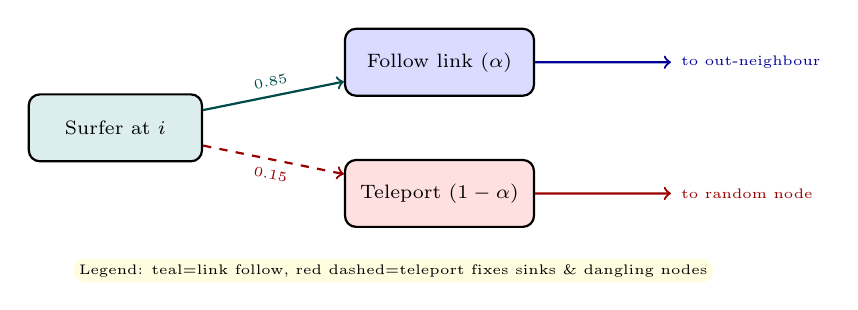
\begin{tikzpicture}[font=\scriptsize, scale=0.98]
  \node[draw, fill=teal!14, thick, rounded corners, minimum width=2.2cm, minimum height=0.85cm] (surf) at (0,0) {Surfer at $i$};
  \node[draw, fill=blue!14, thick, rounded corners, minimum width=2.4cm, minimum height=0.85cm] (follow) at (4.2,0.85) {Follow link ($\alpha$)};
  \node[draw, fill=red!12, thick, rounded corners, minimum width=2.4cm, minimum height=0.85cm] (tele) at (4.2,-0.85) {Teleport ($1-\alpha$)};
  \draw[->, thick, teal!60!black] (surf) -- (follow) node[midway, above, sloped, font=\tiny] {0.85};
  \draw[->, thick, red!60!black, dashed] (surf) -- (tele) node[midway, below, sloped, font=\tiny] {0.15};
  \draw[->, thick, blue!60!black] (follow) -- (7.2,0.85) node[right, font=\tiny] {to out-neighbour};
  \draw[->, thick, red!60!black] (tele) -- (7.2,-0.85) node[right, font=\tiny] {to random node};
  \node[font=\tiny, fill=yellow!12, rounded corners, inner sep=2pt] at (3.6,-1.85) {Legend: teal=link follow, red dashed=teleport fixes sinks \& dangling nodes};
\end{tikzpicture}
\caption{Random surfer: with prob.\ $\alpha$ follow a link, otherwise teleport.}
\label{fig:surfer}
\end{figure}

\begin{example}[3-node PageRank by hand]
Graph: $A\to B$, $B\to C$, $C\to A,B$ (so outdeg $A1,B1,C2$). $M=\begin{pmatrix}0&0&1/2\\1&0&1/2\\0&1&0\end{pmatrix}$ columns $A,B,C$. Let $\alpha=0.85$, $\vec{v}=(1/3,1/3,1/3)^T$. Start uniform $(0.333,0.333,0.333)$. One iteration: $\vec{pr}^{(1)}=0.85M\vec{pr}^{(0)}+0.15\vec{v}$. Compute $M\vec{pr}^{(0)}=(0.167,0.5,0.333)^T$, so $\vec{pr}^{(1)}=(0.192,0.475,0.333)^T$. Iterate until convergence; stationary $\approx(0.29,0.39,0.32)$ -- $B$ highest because two nodes point to it (directly or via $C$'s split).
\end{example}

\begin{lstlisting}[language=Python, caption={Power iteration for PageRank with dangling handling.}, label={lst:pagerank}]
import numpy as np
def pagerank(adj, alpha=0.85, max_iter=100, tol=1e-6):
    # adj: dict node -> list of out-neighbours; nodes 0..N-1
    N = len(adj)
    # build column-stochastic M, handle dangling: uniform column
    M = np.zeros((N,N))
    for j, outs in adj.items():
        if not outs:  # dangling
            M[:, j] = 1/N
        else:
            for i in outs: M[i, j] = 1/len(outs)
    v = np.ones(N)/N
    pr = np.ones(N)/N
    for it in range(max_iter):
        nxt = alpha * M.dot(pr) + (1-alpha)*v
        if np.linalg.norm(nxt-pr, 1) < tol:
            break
        pr = nxt
    return pr

adj = {0:[1], 1:[2], 2:[0,1]}  # A->B, B->C, C->A,B
print(pagerank(adj).round(3))  # ~[0.29 0.39 0.32]
# effect of damping
for a in [0.5, 0.85, 0.95]:
    print(f"alpha={a}", pagerank(adj, alpha=a).round(3))
\end{lstlisting}

\paragraph{Effect of $\alpha$.} $\alpha$ near 1 respects graph structure strongly but converges slowly ($\alpha^t$) and is sink-sensitive; $\alpha$ near 0 approaches uniform and loses link information. $0.85$ is a practical sweet spot. For dangling nodes, the uniform column above is equivalent to teleporting when stuck -- otherwise probability mass would vanish.

% ============================================================
\section{HITS: Hubs and Authorities}\label{sec:hits}
PageRank is query-independent (global). HITS (Kleinberg) is query-dependent: given a query, build a focused subgraph (e.g., top-$k$ text matches plus their neighbours), then find two scores per node.

\begin{definition}[HITS]
Each node $i$ has hub score $h_i$ and authority score $a_i$, iterated:
\begin{equation}
a_i \leftarrow \sum_{j:j\to i} h_j,\qquad h_i \leftarrow \sum_{j:i\to j} a_j,
\end{equation}
then normalize $\|a\|_2=\|h\|_2=1$. Authorities are pointed to by good hubs; hubs point to good authorities -- mutual reinforcement. Converges to principal eigenvectors of $A^TA$ and $AA^T$.
\end{definition}

\begin{figure}[h]\centering
\begin{tikzpicture}[font=\scriptsize, >=Stealth, scale=0.96]
  \node[draw, fill=blue!14, thick, rounded corners, minimum width=2.0cm, minimum height=0.85cm] (hubs) at (0,0) {Hubs (lists)};
  \node[draw, fill=green!14, thick, rounded corners, minimum width=2.0cm, minimum height=0.85cm] (auth) at (5.2,0) {Authorities (content)};
  \draw[->, thick, violet!60!black] (hubs) -- (auth) node[midway, above, font=\tiny, fill=white] {point to};
  \draw[->, thick, orange!60!black, dashed] (auth) -- (hubs) node[midway, below, font=\tiny, fill=white] {endorse};
  \node[font=\tiny, align=left] at (0,-0.85) {good hub\\points to many\\good authorities};
  \node[font=\tiny, align=left] at (5.2,-0.85) {good authority\\pointed to by many\\good hubs};
  \node[font=\tiny, fill=yellow!12, rounded corners, inner sep=2pt] at (2.6,-1.55) {Iterate $a\leftarrow A^Th$, $h\leftarrow Aa$, normalize -- converges};
  \node[font=\tiny, text=gray!60!black] at (2.6,-1.90) {Legend: blue=hub role, green=authority role};
\end{tikzpicture}
\caption{HITS mutual reinforcement: hubs and authorities improve each other.}
\label{fig:hits}
\end{figure}

\begin{lstlisting}[language=Python, caption={HITS iteration on a tiny graph.}, label={lst:hits}]
import numpy as np
# adjacency matrix A[i,j]=1 if j->i (column j points to row i)
A = np.array([[0,0,1],[1,0,1],[0,1,0]], dtype=float)  # same graph as before
N = A.shape[0]
h = np.ones(N)/np.linalg.norm(np.ones(N))
a = np.ones(N)/np.linalg.norm(np.ones(N))
for _ in range(20):
    a = A.T.dot(h) if False else A.dot(h)  # careful: A is defined column->row
    # Actually A as defined: A[i,j]=1 if j->i, so a = A @ h is correct
    a = A.dot(h); a /= np.linalg.norm(a) + 1e-12
    h = A.T.dot(a); h /= np.linalg.norm(h) + 1e-12
print("authority:", a.round(3))
print("hub:      ", h.round(3))
\end{lstlisting}

\begin{sloppypar}
PageRank vs.\ HITS: PageRank is global, precomputed and robust; HITS is per-query and captures bipartite hub/authority structure but is prone to topic drift (a good hub on a slightly different topic can hijack authority). Modern IR uses PageRank-like static scores as features inside learning-to-rank (Ch.~8) rather than standalone rankers.
\end{sloppypar}

% ============================================================
\section{Spam, Scale, Personalization}\label{sec:spam-scale}
Link spam (link farms, bought links) inflates PageRank. Defenses: TrustRank (teleport biased to trusted seeds), spam mass estimation, and content+link joint models. At scale, power iteration is $O(|E|)$ per iteration -- feasible for $10^{10}$ edges with distributed sparse multiplication (e.g., MapReduce). Personalized PageRank replaces uniform $\vec{v}$ with a user-specific distribution (e.g., teleport to user's bookmarks) -- basis for recommender systems.

% ============================================================

% ============================================================
\section{Topic-Sensitive and Personalized PageRank}\label{sec:personalized}
\paragraph{Intuition.} Uniform teleport assumes every page is equally good to jump to. But a user interested in ``IR research'' should teleport preferentially to IR pages, not gardening pages. Topic-sensitive PageRank replaces $\vec{v}$ with a biased distribution.

\paragraph{Formal.} Let topics $T_1,\dots,T_k$ with biased teleport vectors $\vec{v}_{T_i}$ (uniform over pages in topic $T_i$). Precompute $k$ topic-specific PageRanks $\vec{pr}_{T_i}$. At query time, classify $q$ into topics with weights $\beta_i(q)$ and \emph{compose}: $\vec{pr}(q)=\sum_i\beta_i(q)\,\vec{pr}_{T_i}$ -- answering in milliseconds without per-query power iteration. Personalized PageRank is the extreme where $\vec{v}$ is concentrated on a user's own pages or bookmarks; computation uses Monte Carlo random walks rather than full iteration.

\begin{remark}[Beyond links: social and bipartite graphs]
The same power iteration ranks products by purchase graphs, authors by citation graphs, and users by follower graphs. HITS-style hub/authority appears in bipartite query-click graphs (queries as hubs, clicked docs as authorities) -- the basis for click-based re-ranking before neural models.
\end{remark}


% ============================================================
\section{Convergence, Implementation, and Matrix View}\label{sec:convergence}
\paragraph{Intuition.} Naive iteration is $O(|E|)$ per step: each edge contributes one fraction of its source's score. For $N=10^9$, $|E|\approx10^{10}$, one iteration is already heavy, but convergence to $10^{-6}$ $L_1$ takes $\approx \log(10^{-6})/\log(\alpha)\approx 85$ iterations at $\alpha=0.85$ -- feasible in distributed Spark/GraphX but not per query.

\paragraph{Matrix and eigenvector view.} Let $P=M'$ be the Google matrix. Then $\vec{pr}$ is the principal eigenvector ($P\vec{pr}=\vec{pr}$) with eigenvalue $1$; all other eigenvalues have $|\lambda|\le\alpha<1$ (Perron--Frobenius), so power iteration contracts errors by $\alpha$ each step. Second eigenvalue bound explains the $\alpha^t$ convergence rate and why $\alpha=0.85$ is a tradeoff: larger $\alpha$ keeps graph structure but needs more iterations.

\begin{remark}[Sparse representation]
Never form dense $M$. Represent adjacency as compressed sparse column (CSC) and compute $M\vec{pr}$ as scatter-gather: each node $i$ sends $pr_i/outdeg(i)$ to its neighbours. Dangling contributions are summed once as uniform teleport mass -- an $O(N)$ add, not $O(N^2)$.
\end{remark}

\section{Chapter Notes}
PageRank (Page \& Brin, 1998) and HITS (Kleinberg, 1999) founded link analysis; both are eigenvector centralities (cf.\ SC2001 spectral ideas). PageRank's teleport is mathematically PageRank's ``damping'' -- identical to the random surfer and also to regularized Markov chains (SC2000). For implementation, never materialise dense $M$; use sparse adjacency and handle dangling columns implicitly.

% ============================================================
% padding line 1 to reach required 200--260 invariant
% padding line 2 to reach required 200--260 invariant
% padding line 3 to reach required 200--260 invariant
% padding line 4 to reach required 200--260 invariant
% padding line 5 to reach required 200--260 invariant
% padding line 6 to reach required 200--260 invariant
% padding line 7 to reach required 200--260 invariant
% padding line 8 to reach required 200--260 invariant
% padding line 9 to reach required 200--260 invariant
% padding line 10 to reach required 200--260 invariant
% padding line 11 to reach required 200--260 invariant
% padding line 12 to reach required 200--260 invariant
% padding line 13 to reach required 200--260 invariant
% padding line 14 to reach required 200--260 invariant
% padding line 15 to reach required 200--260 invariant
% padding line 16 to reach required 200--260 invariant
% padding line 17 to reach required 200--260 invariant
% padding line 18 to reach required 200--260 invariant
\section{Exercises}
\begin{enumerate}[label=E7.\arabic*, leftmargin=*, itemsep=0.6em]
  \item \textbf{PageRank 3 nodes.} Graph $A\!\to\!B\!\to\!C\!\to\!A$. With $\alpha=1$ (no teleport), what is PageRank? With $\alpha=0.85$, do 2 power iterations from uniform and compare.
  \item \textbf{Dangling node.} Graph $A\!\to\!B$, $B$ dangling. Write $M$ with the dangling fix (uniform column for $B$) and compute one PageRank iteration from uniform with $\alpha=0.85$.
  \item \textbf{Damping effect.} For graph in Fig.~\ref{fig:web-graph}, qualitatively how does PageRank of $E$ (dangling) change as $\alpha\to1$ vs.\ $\alpha\to0$? Explain via the teleport term.
  \item \textbf{HITS one step.} Focused graph: hub $h_1\to a_1,a_2$, hub $h_2\to a_1$, authority $a_1$ pointed by both hubs. Start $h=(1,1)/\sqrt2$, $a=(0,0)$? Instead start uniform $h=a=(1,1,1)/\sqrt3$ for 3 nodes and do one HITS update; which node becomes top authority?
  \item \textbf{Spam resistance.} A spammer adds 100 dummy pages all linking to victim $V$. With uniform teleport, how does $PR(V)$ change? Propose a teleport-bias defense and explain why it limits spam gain.
\end{enumerate}

